% Figure from MATH 591 notes, Assignment 9 Problem 2(c): from the submitted solution (sphere minus a meridian, chart image)
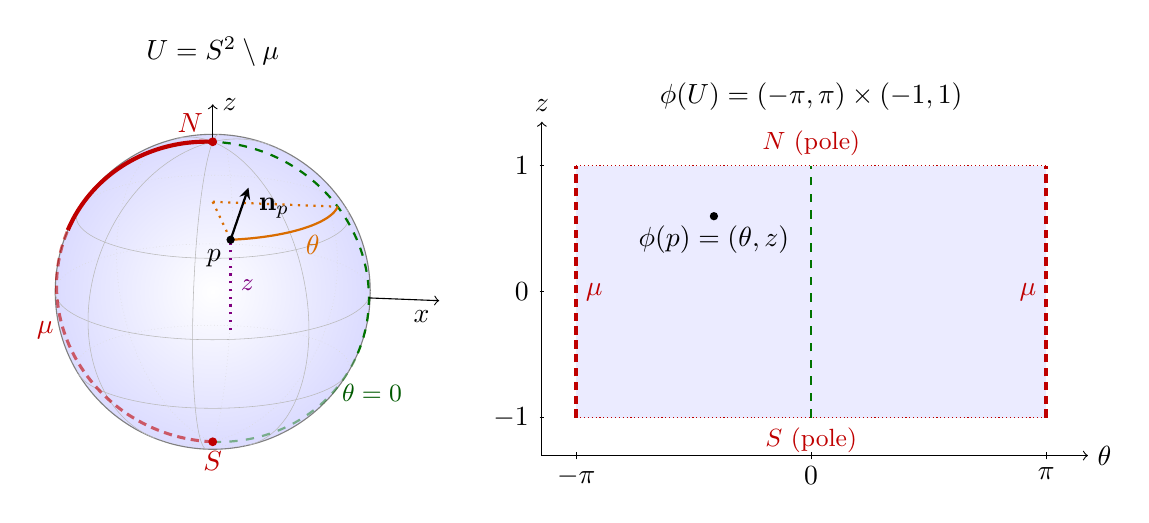
\begin{tikzpicture}[lat/.style={gray!55, very thin}, latback/.style={gray!30, very thin, densely dotted}, greenwich/.style={green!45!black, thick, dashed}, mu/.style={red!75!black, line width=1.5pt}, muback/.style={red!75!black, line width=1.1pt, densely dashed, opacity=0.6}]
% the sphere (orthographic projection)
\shade[inner color=white, outer color=blue!14] (0,0) circle (2.0cm);
\draw[gray] (0,0) circle (2.0cm);
\begin{scope}[x={(1.984cm,-0.078cm)}, y={(0.256cm,0.604cm)}, z={(-0.000cm,1.905cm)}]
\draw[latback] plot[domain=-180.0:-162.0, samples=72, smooth, variable=\t] ({0.8660*cos(\t)}, {0.8660*sin(\t)}, -0.5);
\draw[lat] plot[domain=-162.0:-3.2, samples=72, smooth, variable=\t] ({0.8660*cos(\t)}, {0.8660*sin(\t)}, -0.5);
\draw[latback] plot[domain=-3.2:180.0, samples=72, smooth, variable=\t] ({0.8660*cos(\t)}, {0.8660*sin(\t)}, -0.5);
\draw[latback] plot[domain=-180.0:-172.6, samples=72, smooth, variable=\t] ({1.0000*cos(\t)}, {1.0000*sin(\t)}, 0);
\draw[lat] plot[domain=-172.6:7.4, samples=72, smooth, variable=\t] ({1.0000*cos(\t)}, {1.0000*sin(\t)}, 0);
\draw[latback] plot[domain=7.4:180.0, samples=72, smooth, variable=\t] ({1.0000*cos(\t)}, {1.0000*sin(\t)}, 0);
\draw[lat] plot[domain=-180.0:18.0, samples=72, smooth, variable=\t] ({0.8660*cos(\t)}, {0.8660*sin(\t)}, 0.5);
\draw[latback] plot[domain=18.0:176.8, samples=72, smooth, variable=\t] ({0.8660*cos(\t)}, {0.8660*sin(\t)}, 0.5);
\draw[lat] plot[domain=176.8:180.0, samples=72, smooth, variable=\t] ({0.8660*cos(\t)}, {0.8660*sin(\t)}, 0.5);
\draw[latback] plot[domain=-90.0:-62.3, samples=36, smooth, variable=\t] ({cos(\t)*cos(-135)}, {cos(\t)*sin(-135)}, {sin(\t)});
\draw[lat] plot[domain=-62.3:90.0, samples=36, smooth, variable=\t] ({cos(\t)*cos(-135)}, {cos(\t)*sin(-135)}, {sin(\t)});
\draw[latback] plot[domain=-90.0:-72.1, samples=36, smooth, variable=\t] ({cos(\t)*cos(-90)}, {cos(\t)*sin(-90)}, {sin(\t)});
\draw[lat] plot[domain=-72.1:90.0, samples=36, smooth, variable=\t] ({cos(\t)*cos(-90)}, {cos(\t)*sin(-90)}, {sin(\t)});
\draw[latback] plot[domain=-90.0:-68.0, samples=36, smooth, variable=\t] ({cos(\t)*cos(-45)}, {cos(\t)*sin(-45)}, {sin(\t)});
\draw[lat] plot[domain=-68.0:90.0, samples=36, smooth, variable=\t] ({cos(\t)*cos(-45)}, {cos(\t)*sin(-45)}, {sin(\t)});
\draw[latback] plot[domain=-90.0:62.4, samples=36, smooth, variable=\t] ({cos(\t)*cos(45)}, {cos(\t)*sin(45)}, {sin(\t)});
\draw[lat] plot[domain=62.4:90.0, samples=36, smooth, variable=\t] ({cos(\t)*cos(45)}, {cos(\t)*sin(45)}, {sin(\t)});
\draw[latback] plot[domain=-90.0:72.2, samples=36, smooth, variable=\t] ({cos(\t)*cos(90)}, {cos(\t)*sin(90)}, {sin(\t)});
\draw[lat] plot[domain=72.2:90.0, samples=36, smooth, variable=\t] ({cos(\t)*cos(90)}, {cos(\t)*sin(90)}, {sin(\t)});
\draw[latback] plot[domain=-90.0:68.0, samples=36, smooth, variable=\t] ({cos(\t)*cos(135)}, {cos(\t)*sin(135)}, {sin(\t)});
\draw[lat] plot[domain=68.0:90.0, samples=36, smooth, variable=\t] ({cos(\t)*cos(135)}, {cos(\t)*sin(135)}, {sin(\t)});
\draw[greenwich, opacity=0.45] plot[domain=-90.0:-21.8, samples=36, smooth, variable=\t] ({cos(\t)}, 0, {sin(\t)});
\draw[greenwich] plot[domain=-21.8:90.0, samples=36, smooth, variable=\t] ({cos(\t)}, 0, {sin(\t)});
\draw[muback] plot[domain=-90.0:21.9, samples=36, smooth, variable=\t] ({-cos(\t)}, 0, {sin(\t)});
\draw[mu] plot[domain=21.9:90.0, samples=36, smooth, variable=\t] ({-cos(\t)}, 0, {sin(\t)});
% axes
\draw[->] (1,0,0) -- (1.45,0,0) node[anchor=north east] {$x$};
\draw[->] (0,0,1) -- (0,0,1.25) node[anchor=west] {$z$};
% poles and labels
\fill[red!75!black] (0,0,1) circle (1.6pt) node[anchor=south east] {$N$};
\fill[red!75!black] (0,0,-1) circle (1.6pt) node[anchor=north] {$S$};
\node[red!75!black, anchor=east] at ({-cos(-17)}, 0, {sin(-17)}) {$\mu$};
\node[green!35!black, anchor=west, font=\small] at ({cos(-40)}, 0, {sin(-40)}) {$\theta = 0$};
% the point p, its coordinates, and the normal
\coordinate (p) at ({0.8000*cos(-74.5)}, {0.8000*sin(-74.5)}, 0.6);
\draw[orange!85!black, dotted, thick] (0,0,0.6) -- (p);
\draw[orange!85!black, dotted, thick] (0,0,0.6) -- (0.8000,0,0.6);
\draw[orange!85!black, thick] plot[domain=0:-74.5, samples=30, smooth, variable=\t] ({0.8000*cos(\t)}, {0.8000*sin(\t)}, 0.6);
\node[orange!85!black, anchor=north west, inner sep=1pt] at ({0.8000*cos(-37.2)}, {0.8000*sin(-37.2)}, 0.58) {$\theta$};
\draw[violet, dotted, thick] ({0.8000*cos(-74.5)}, {0.8000*sin(-74.5)}, 0) -- node[anchor=west, font=\small] {$z$} (p);
\draw[-stealth, thick] (p) -- ({2.0*0.8000*cos(-74.5)}, {2.0*0.8000*sin(-74.5)}, 1.2) node[anchor=north west] {$\mathbf{n}_p$};
\fill (p) circle (1.5pt) node[anchor=north east] {$p$};
\end{scope}
\node at (0,3.05) {$U = S^2 \setminus \mu$};
% the chart image
\begin{scope}[xshift=7.6cm, x=0.95cm, y=1.6cm]
\fill[blue!8] (-3.1416,-1) rectangle (3.1416,1);
\draw[red!75!black, line width=1.3pt, densely dashed] (-3.1416,-1) -- (-3.1416,1);
\draw[red!75!black, line width=1.3pt, densely dashed] (3.1416,-1) -- (3.1416,1);
\draw[red!75!black, densely dotted] (-3.1416,1) -- node[above, font=\small] {$N$ (pole)} (3.1416,1);
\draw[red!75!black, densely dotted] (-3.1416,-1) -- node[below, font=\small] {$S$ (pole)} (3.1416,-1);
\draw[green!45!black, thick, dashed] (0,-1) -- (0,1);
\node[red!75!black, anchor=west] at (-3.1416,0) {$\mu$};
\node[red!75!black, anchor=east] at (3.1416,0) {$\mu$};
\fill (-1.3,0.6) circle (1.5pt) node[anchor=north] {$\phi(p) = (\theta, z)$};
\draw[->] (-3.6,-1.3) -- (3.7,-1.3) node[anchor=west] {$\theta$};
\draw[->] (-3.6,-1.3) -- (-3.6,1.35) node[anchor=south] {$z$};
\foreach \x/\l in {-3.1416/-\pi, 0/0, 3.1416/\pi} \draw (\x,-1.33) -- (\x,-1.27) node[below=2pt] {$\l$};
\foreach \y in {-1, 0, 1} \draw (-3.63,\y) -- (-3.57,\y) node[left=2pt] {$\y$};
\node at (0,1.55) {$\phi(U) = (-\pi, \pi) \times (-1, 1)$};
\end{scope}
\end{tikzpicture}
